\usetikzlibrary{arrows.meta}
\begin{tikzpicture}[x=1cm,y=1cm,line width=.6pt,>=Stealth,font=\normalsize]
\coordinate (H) at (1.2,0);
\coordinate (O) at (0,0);
\coordinate (C) at (0,1.2);
\coordinate (X1) at (2.05,0);
\coordinate (V0) at (1.2,-0.32);
\coordinate (V1) at (1.2,2.56);
\draw[->] (O) -- (X1);
\draw (C) circle[radius=1.2cm];
\draw (V0) -- (V1);
\node[anchor=north east,inner sep=0pt,xshift=-2pt,yshift=-2pt] at (O) {$O$};
\node[anchor=west,inner sep=0pt,xshift=2pt] at (X1) {$x$};
\node[anchor=south west,inner sep=0pt,xshift=4pt,yshift=3pt] at (H) {$\dfrac{1}{2}$};
\end{tikzpicture}
